\section{Modèles théoriques}
Nous avons présenté brièvement dans le chapitre~\ref{chap:rw:supervision} que les systèmes de gestions de flux de données s'inspiraient du modèle relationnel. Le modèle relationnel ne supporte toutefois pas le dynamisme des données. Ainsi de nombreuses propositions ont été faites dans l'état de l'art pour reconstruire un modèle tout en tentant de réutiliser les connaissances développées sur les systèmes de gestion de base de données relationnels depuis 40 ans.

\TODO{plan}

\subsection{Les premiers modèles}

\subsubsection{La genèse de la gestion de flux}
L'idée de créer des requêtes continues a été présenté en 1992 dans le système Tapestry~\cite{Terry:tapestry}. Dans ce système une requête continue est avant tout une requête instantanée, mais la sémantique étant que celle-ci sera exécuté périodiquement. Ces requêtes s'appliquent sur un ensemble de données sans suppression ou mise à jour (\textit{append-only}). Le résultat de cette requête sera représenté par le flux des nouvelles données calculés de manière incrémental. Pour cela, les relations sont réellement considérés comme des variables et elles deviennent donc dépendantes du temps.

En 1995, les flux de données ont été explorés tout d'abord par le modèle séquentiel $\mathcal{SEQ}$~\cite{Seshadri:seq}. Dans ce modèle, une \enquote{\it séquence} est un ensemble d'enregistrements (n-uplets relationnels) avec un ordre positionnel. Dans le modèle relationnel originel~\cite{Codd:model}, ceci n'est pas autorisé car l'ordre des n-uplets est dit \enquote{\it irrelevant}. La sémantique de spécification des opérateurs relationnels utilise cet liberté d'ordre pour être consistent et obtenir des propriétés intéressantes (voir chapitre~\ref{chap:contrib:astral}). Ici, le formalisme de $\mathcal{SEQ}$ montre qu'il est toujours possible d'exploiter les opérateurs algébriques classiques et que de nouveaux peuvent être créés comme les premières notions de regroupements d'n-uplets appelées \textit{collapse}\footnote{Cette primitive représente ce qui deviendra l'opérateur de fenêtrage plus tard}. Ce formalisme a été fondateur pour plusieurs travaux futurs qui s'inspirent explicitement de ce modèle~\cite{Gurgen:sens,Babcock:issues}.

Par la suite, les premières opérations sur les flux en tant que tels ont pu apparaître avec le système Chronicle~\cite{Jagadish:chronicle}. Toutefois, les flux étaient considérés soit comme un ensemble de données historique, soit comme une données constamment mise à jour (fenêtres complète, ou instantanée). La notion de fenêtre a été présenté pour la première fois dans Tribeca~\cite{Sullivan:tribeca,Sullivan:tribeca2}. Sa spécification était basée sur sa taille positionnelle (nombre de données) ou temporelle (durée). Toutefois, ce système ne pouvait gérer qu'un seul flux à la fois. La notion de fenêtre sera par la suite intégrée à SQL:1999~\cite{Melton:sql1999} ainsi que dans SQL:2003~\cite{Eisenberg:sql2003} pour des opérations OLAP.

Les requêtes continues ont été aussi développés grâce aux besoins de plus en plus demandant des bases de données en constante évolution. Lors de la fin de années 90, les bases de données contenant des pages et flux web dynamiques ont de graves problèmes de performances pour analyser les flux d'événements. Ceci débouchera sur des projets tels que OpenCQ~\cite{Liu:opencq} et surtout NiagaraCQ~\cite{Chen:niagaracq} qui permettent de faire notamment des opérations de jointures.

Le début des années 2000 a marqué l'avènement des systèmes de gestion de flux de données à part entière. Cela a notamment été motivé par l'arrivée d'applications réseaux~\cite{Cranor:gigascope} et capteurs~\cite{Madden:tag,Yao:cougar} demandeurs de plus en plus de puissance d'expression ainsi que de performances. A quelques mois d'intervalles, les premiers SGFD ont donc fait leur apparition : TelegraphCQ~\cite{Chandrasekaran:telegraphcq} et Aurora~\cite{Carney:monitoring} et STREAM~\cite{Widom:queries}. Ce dernier apporte de plus son algèbre : SQuAl~\cite{Abadi:aurora}. Celle-ci sera la première algèbre complète sur les flux de données. Un flux est considéré comme un ensemble de n-uplets strictement ordonnés avec un schéma prédéfinit $(\textbf{TS}, A_1,\dots, A_n)$, où $\textbf{TS}$ correspond au \textit{timestamp}. L'algèbre décrit le comportement d'opérateurs simples comme la sélection (\textit{Filter}), la projection-évaluation (\textit{Map}) et l'union (\textit{Union}). Mais aussi d'opérateurs complexes (i.e. utilisant une fenêtre) tels que le tri à la volée (\textit{BSort}), l'agrégat (\textit{Aggregate}), la jointure sur bande (\textit{Join}) et un opérateur de synchronisation de \textit{timestamp} (\textit{Resample}). Il est important de voir que ces opérateurs complexes se définissent grâce à des fenêtres prédéfinies à l'avance. 

TelegraphCQ~\cite{Chandrasekaran:telegraphcq} quant à lui proposait un langage de requête beaucoup plus axé sur le relationnel avec notamment une définition de fenêtre générique. En effet ces dernières étaient décrites par une séquence de type \textit{boucle for}.
\begin{center}
\begin{minipage}[c]{0.75\textwidth}
\begin{verbatim}
for(t=initial_value; continue_condition(t); change(t)) {
    WindowIs(StreamA, left_end(t), right_end(t));
    WindowIs(StreamB, left_end(t), right_end(t)); …
}
\end{verbatim}
\end{minipage}
\end{center}

Cependant, depuis le début des requêtes continues, la spécification des opérateurs étaient avant tout dirigés par l'implémentation. Cela a amené a des limitations d'expressivité (voire même des divergences d'interprétation). Ceci a été notamment traité dans le SGFD générique STREAM.

\subsection{La sémantique abstraite à deux concepts}
Le système STREAM~\cite{Widom:queries, Arasu:stream} se démarque des autres systèmes de son époque pour avoir décrit une sémantique abstraite à deux concepts~\cite{Arasu:semantic} :
\begin{itemize}
 \item[\textbf{Un flux}] est un ensemble potentiellement infini d'n-uplets conformes à un schéma commun possédant un \textit{timestamp}.
 \item[\textbf{Une relation}] Une relation est une fonction qui associe le temps à un ensemble fini d'n-uplets conformes à un schéma commun.
\end{itemize}
Le point crucial de cette approche est le fait que les opérateurs sont capables de passer d'un concept à l'autre (voir figure~\ref{fig:rw:sgfd:streamrelation}. Ainsi, les opérateurs capables de traiter des relations pour en fournir une nouvelle sont les opérateurs relationnels. Ceux-ci sont notamment issus de l'algèbre relationnelle usuelle (réadapté pour être conforme formellement au modèle évidemment) tels que $\sigma$, $\Pi$ et même $\Join$. Les opérateurs transformant un flux en relation sont les opérateurs de fenêtres. Les opérateurs transformants les flux en relations sont des \textit{streamers}.
\begin{figure}[ht]
    \centering
    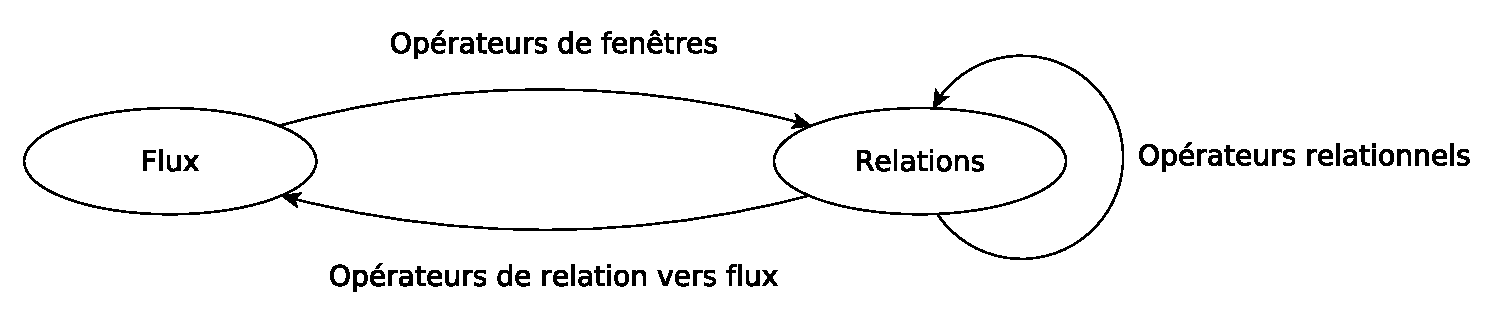
\includegraphics[width=0.75\textwidth]{rw-sgfd-streamrelation}
    \caption{Associations utilisés dans la sémantique abstraite de STREAM}
\end{figure}
\TODO{Exemple de requête}
Le point clé et novateur de cette approche étant que les opérateurs de flux vers flux \textbf{n'existe pas}. Les auteurs ont justifié cette approche car l'écriture de requête était plus intuitive et que cela permettait de généraliser l'utilisation des vues matérialisés dans le traitement des flux (introduit auparavant dans Chronicle). La spécification de cette sémantique a permit par la suite de décrire le langage associé CQL~\cite{Arasu:cql} qui est désormais utilisé dans de nombreux produits académiques et commerciaux~\cite{Witkowski:oraclecq,url:sqlstream}.

% \textbf{Rethinking formal models. }
% Recently, the core basis of  the aforementioned  models has been proven to be semantically ambiguous. Therefore, standardization and clarification of the core semantics of some operators have been proposed~\cite{Jain:spread}.  The concept of {\bf batch} as a set of tuples having the same timestamp, has been introduced. 
% A new wave of formalization arises subsequently  to fill the lack of mathematical models. Some works contribute to more complete  formalization of windows~\cite{Patroumpas:window,Botan:secret,Petit:window} as they are  the aspect  of stream processing which has led to the most different interpretations.


\subsection{Nouvelles formalisations}
